% -*- root: ../Presentation.tex -*-
\section{Status}
\begin{frame}{Status}{}
\begin{figure}
\centering     %%% not \center
\subfigure[Grænseværdier på gamle program]{\label{fig:a}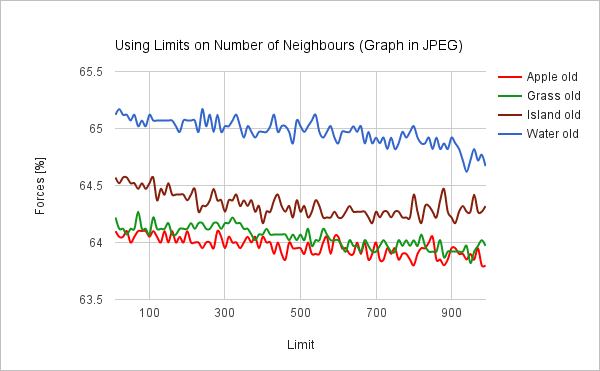
\includegraphics[width=.5\textwidth]{figures/graphOld.png}}
\subfigure[Grænseværdier på nye program]{\label{fig:b}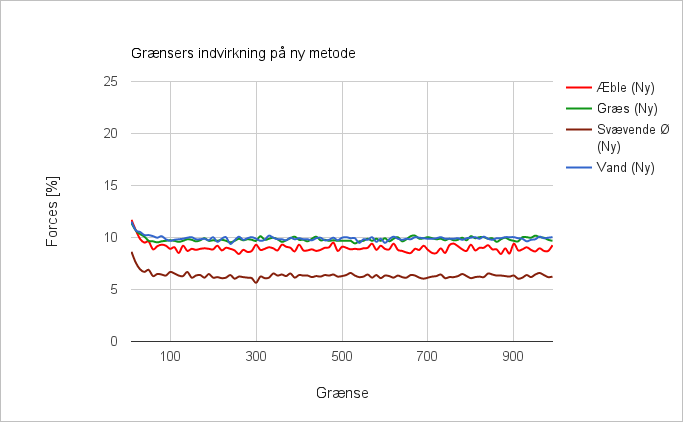
\includegraphics[width=.5\textwidth]{figures/graphNew.png}}
\caption{my caption}
\end{figure}
\end{frame}
\begin{frame}{Status}{}
\begin{figure}
\centering     %%% not \center
\subfigure[]{\label{fig:a}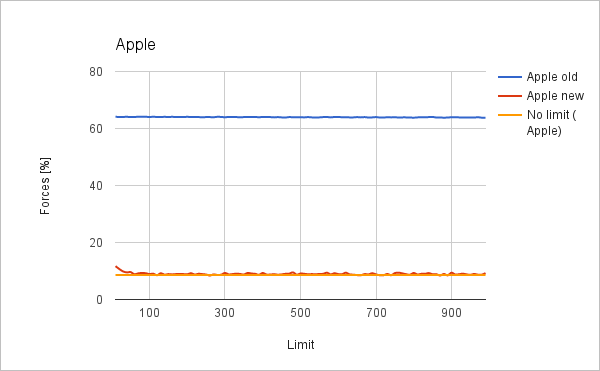
\includegraphics[width=.4\textwidth]{figures/graphApple.png}}
\subfigure[]{\label{fig:b}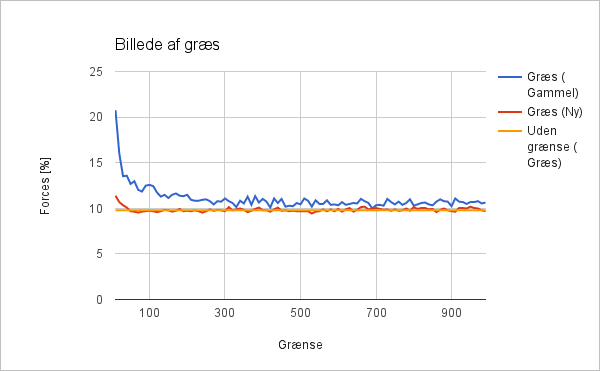
\includegraphics[width=.4\textwidth]{figures/graphGrass.png}}
\subfigure[]{\label{fig:a}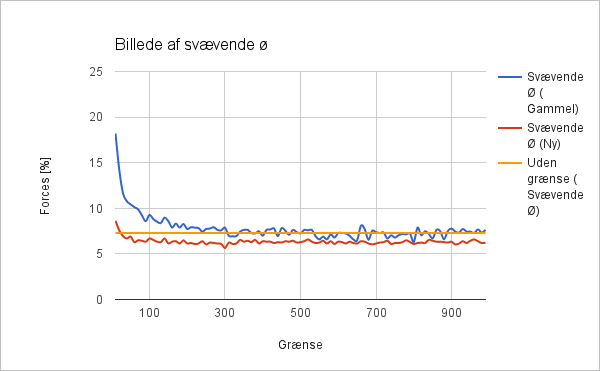
\includegraphics[width=.4\textwidth]{figures/graphIsland.png}}
\subfigure[]{\label{fig:b}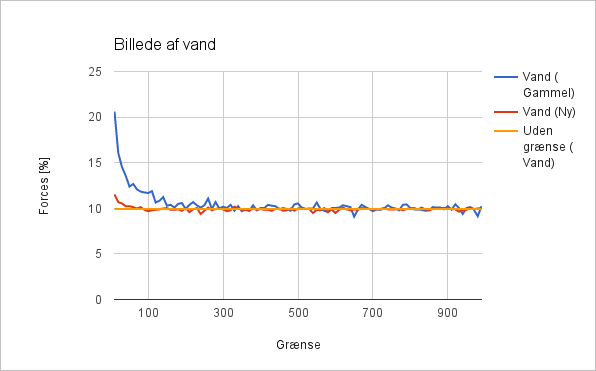
\includegraphics[width=.4\textwidth]{figures/graphWater.png}}
\caption{Sammenligning af grænseværdier}
\label{fig:limits}
\end{figure}
\end{frame}

\begin{frame}{Status}{}
\begin{figure}
\centering     %%% not \center
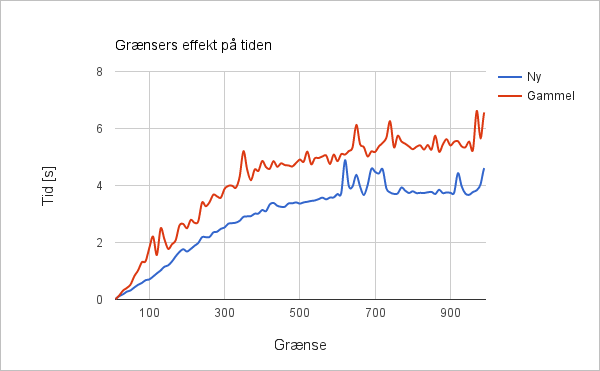
\includegraphics[width=.6\textwidth]{figures/graphTime.png}
\caption{Effekten fra grænseværdier på tiden}
\label{fig:limits}
\end{figure}
\end{frame}
